\documentclass{sig-alternate-05-2015}

\usepackage{multirow}
\usepackage{color}
\usepackage{algorithm}
\usepackage{algorithmic}
\usepackage{mathrsfs}
\DeclareMathOperator*{\argmin}{argmin}
\DeclareMathOperator*{\argmax}{argmax}

\usepackage{url}
\usepackage{hyperref}
\newcommand{\surl}[1]
{
	\urlstyle{same}\url{#1}
}

\usepackage[svgnames]{xcolor}
\definecolor{navy}{rgb}{0.1, 0.1, 0.8}
\definecolor{gray}{rgb}{0.4, 0.4, 0.4}

\usepackage{soul} %% needed for highlighting

% spacing hacks
\newcommand{\captionmoveup}{\vspace{-0.2in}}

\begin{document}


\CopyrightYear{2016}
\setcopyright{acmcopyright}
\conferenceinfo{CIKM'16 ,}{October 24-28, 2016, Indianapolis, IN, USA}
\isbn{978-1-4503-4073-1/16/10}\acmPrice{\$15.00}
\doi{http://dx.doi.org/10.1145/2983323.2983672}

\clubpenalty=10000
\widowpenalty = 10000

\title{Learning Points and Routes to Recommend Trajectories}

\numberofauthors{3}
\author{
    \alignauthor Dawei Chen$^{*\dagger}$\\
    \alignauthor Cheng Soon Ong$^{\dagger *}$\\
    \alignauthor Lexing Xie$^{*\dagger}$\\
    \and
    $^*$The Australian National University, $^\dagger$Data 61, CSIRO, Australia\\
    \and
    \{u5708856, chengsoon.ong, lexing.xie\}@anu.edu.au
}

\maketitle

%!TEX root = main.tex

The problem of recommending tours to travellers is an important and broadly studied area.
Suggested solutions include various approaches of points-of-interest (POI)
recommendation and route planning.
We consider the task of recommending a sequence of POIs 
%as a tour to travellers
, that simultaneously uses information about POIs and routes.
Our approach unifies the treatment of various sources of information
by representing them as features in machine learning algorithms, enabling us to
learn from past behaviour. %without specialised treatment of spatial, temporal or social information.
Information about POIs are used to learn a POI ranking model
that accounts for the start and end points of tours.
Data about previous trajectories are used for learning transition patterns between POIs that
enable us to recommend probable routes.
In addition, a probabilistic model is proposed
%and a Structured Support Vector Machine are used
to combine the results of POI ranking and the POI to POI transitions.
We propose a new F$_1$ score on pairs of POIs
that capture the order of visits.
Empirical results show that our approach improves on
recent methods, and demonstrate that
combining points and routes enables better trajectory recommendations.


\keywords{Trajectory recommendation; learning to rank; planning}

%!TEX root = main.tex

\section{Introduction}
\label{sec:intro}

\begin{figure}[ht]
	\centering
	%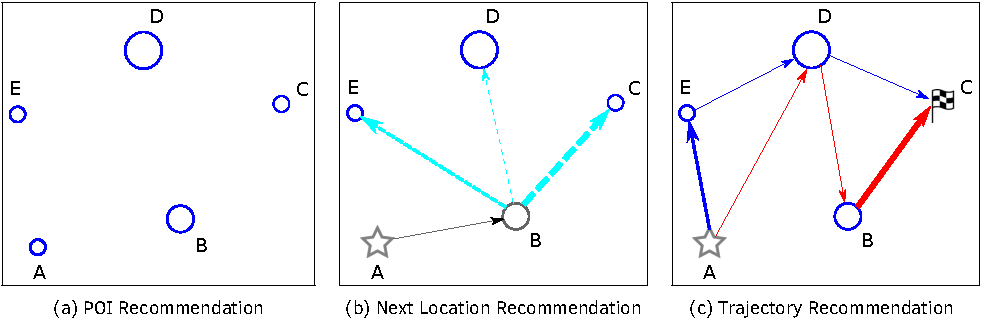
\includegraphics[width=0.7\textwidth]{fig/fig1-flavours.pdf}
	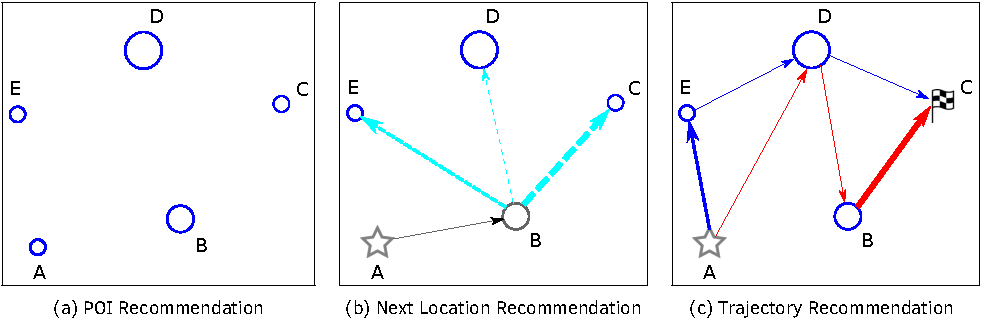
\includegraphics[width=\columnwidth]{fig/fig1-flavours.pdf}
	\caption{Three settings of trajectory recommendation problems. 
Node size: POI score; edge width: transition score between pairs of POIs; 
%grey: input query; 
grey: observed;
star: starting location; flag: ending location. See Section~\ref{sec:intro} for details.
}
	\label{fig:threesettings}
\end{figure}



This paper proposes a novel solution to recommend travel routes in cities.
A large amount of location traces are becoming available from ubiquitous location tracking devices.
For example, FourSquare
%, the local search and discovery service, 
has 50 million monthly users who have made 8 billion check-ins~\cite{4sq},
and Flickr
%, the online photo-sharing site, 
hosts over 2 billion geo-tagged public photos~\cite{flickr}. 
Such large amounts of travel data provide new opportunities for better
travel planning traditionally done with written travel guides.
%for example, choosing and ranking locations for a variety of activities from dining to recreation,
%and potential new solutions to orienteering and routing problems.
Good solutions to these problems will in turn lead to better urban experiences for residents and visitors alike, and foster sharing of even more location-based behavioural data.

\section{POI, Query and Transition}
\label{sec:feature}

The goal of tour recommendation is to suggest a sequence of POIs, $(p_1, \ldots, p_L)$, of length $L$ such that the user's utility is maximised. The user provides the desired start ($p_1=p_s$) and end point ($p_L=p_e$), as well as the number $L$ of POIs desired, from which we propose a trajectory through the city.
The training data consists of a set of tours of varying length in a particular city.
We consider only POIs that have been visited by at least one user in the past, and
construct a graph with POIs as nodes and directed edges representing the observed transitions between pairs of POIs in tours. 


We extract the category, popularity (number of distinct visitors)~\cite{ht10}, total number of visits and average visit duration for each POI.
POIs are grouped into $5$ clusters using K-means according to their geographical locations to reflect their neighbourhood.
Furthermore, since we are constrained by the fact that trajectories have to be of length $L$ and start and end at certain points, we hope to improve the recommendation by using this information.
In other words, we use the \textit{query} $q = (p_s, p_e, L)$ to construct new features by contrasting candidate POIs with $p_s$ and $p_e$.
For each of the POI features (category, neighbourhood, popularity, total visits and average duration),
we construct two new features by taking the difference of the feature in POI $p$ with $p_s$ and $p_e$ respectively.
For the category (and neighbourhood), we set the feature to $1$ when their categories (and cluster identities) are the same and $-1$ otherwise.
For popularity, total visits and average duration, we take the real valued difference.
Lastly, we compute the distance from POI $p$ to $p_s$ (and $p_e$) using the Haversine formula~\cite{haversine},
and also include the required length $L$.


\begin{figure}[t]
\includegraphics[width=\columnwidth]{fig/poi_transmat.png}
\caption{Transition matrices for two POI features from Melbourne: POI category and neighbourhood.
}
\label{fig:transmat}\captionmoveup
\end{figure}


In addition to information about each individual POI, a tour recommendation system would benefit
from capturing the likelihood of going from one POI to another different POI. One option would be to
directly model the probability of going from any POI to any other POI, but this has several weaknesses:
Such a model would be unable to handle a new POI (one that has not yet been visited),
or pairs of existing POIs that do not have an observed transition.
Furthermore, even if we restrict ourselves to known POIs and transitions,
there may be locations which are rarely visited,
leading to significant challenges in estimating the probabilities from empirical data.

We model POI transitions using a Markov chain with discrete 
states by factorising the transition probability ($p_i$ to $p_j$) 
as a product of transition probabilities between pairs of individual POI features, 
assuming independence between these feature-wise transitions.
The popularity, total visits and average duration are discretised by binning
them uniformly into $5$ intervals on the log scale.
These feature-to-feature transitions are estimated from data using maximum likelihood principle.
The POI-POI transition probabilities can be efficiently computed by taking the Kronecker product of 
transition matrices for the individual features,
and then updating it based on three additional constraints as well as appropriate normalisation.
First we disallow self-loops by setting the probability of ($p_i$ to $p_i$) to zero.
Secondly, when multiple POIs have identical (discretised) features, we distribute the probability uniformly among POIs in the group.
Third, we remove feature combinations that has no POI in dataset. 
Figure~\ref{fig:transmat} visualises the transition matrices for two POI features, category and neighbourhood, in Melbourne.

\section{Tour Recommendation}
\label{sec:recommendation}

In this section, we first describe the recommendation of points and routes,
then we discuss how to combine them, and finally we propose a method to avoid sub-tours.

\subsection{POI Ranking and Route Planning}
\label{sec:rankplan}

A naive approach would be to recommend trajectories based on the popularity of POIs only,
that is we always suggest the top-$k$ most popular POIs for all visitors given the start and end location.
We call this baseline approach \textsc{PoiPopularity},
and its only adaptation to a particular query is to adjust $k$ to match the desired length.

On the other hand, we can leverage the whole set of POI features described in Section~\ref{sec:feature}
to learn a ranking of POIs using rankSVM, with linear kernel and L$2$ loss~\cite{lranksvm},
\begin{equation*}
\min_{\mathbf{w}} \frac{1}{2}
                  \mathbf{w}^T \mathbf{w} +
                  \underset{p_i, p_j \in \mathcal{P},~ q \in \mathcal{Q}}{C ~\sum}
                  \max \left( 0,~ 1 - \mathbf{w}^T (\phi_{i,q} - \phi_{j,q}) \right)^2,
\end{equation*}
where $\mathbf{w}$ is the parameter vector,
$C > 0$ is a regularisation constant,
$\mathcal{P}$ is the set of POIs to rank,
$\mathcal{Q}$ denotes the queries corresponding to trajectories in training set,
and $\phi_{i,q}$ is the feature vector for POI $p_i$ with respect to query $q$. 
The ranking score of $p_i$ given query $q$ is computed as $R_{i,q} =\mathbf{w}^T \phi_{i,q}$. 

For training the rankSVM, the labels are generated using the number of occurrences of
POI $p$ in trajectories grouped by query $(p_s, p_e, L)$,
without counting the occurrence of $p$ when it is the origin or destination of a trajectory.
Our algorithm, \textsc{PoiRank}, recommends a trajectory for a particular query
by first ranking POIs then takes the top ranked $L-2$ POIs and connects them according to the ranks.


In addition to recommend trajectory by ranking POIs, we can leverage the POI-POI transition probabilities and
recommend a trajectory (with respect to a query) by maximising the transition likelihood.
The maximum likelihood of the Markov chain of transitions is found using a variant of the Viterbi algorithm (with uniform emission probabilities).
We call this approach that only uses the transition probabilities between POIs as \textsc{Markov}.


\subsection{Combine Ranking and Transition}
\label{sec:rank+markov}

We would like to leverage both point ranking and transitions,
i.e., recommending a trajectory that maximises the points ranking of its POIs as well as its transition likelihood at the same time.
To begin with, we transform the ranking scores $R_{j,q}$ of POI $p_j$ with respect to query $q$
to a probability distribution using the softmax function,
\begin{equation}
\label{eq:rankprob}
P_R(p_j | q) = \frac{\exp(R_{j,q})}{\sum_i \exp(R_{i,q})},
\end{equation}
One option to find a trajectory that simultaneously maximises the ranking probabilities of its POIs and its transition likelihood is to optimise the following objective:
\vspace{-0.3em}
\begin{equation*}
    \argmax_{\mathcal{T} \in \mathcal{P}^L} ~\alpha \sum_{k=2}^{L} \log P_R(p_{k} | q) +
                                     (1-\alpha) \sum_{k=1}^{L-1} \log P(p_{k+1} | p_{k}),
\end{equation*}
such that
$p_{1} = p_s, ~ p_{L} = p_e$ and
$p_{k} \in \mathcal{P}, ~1 \le k \le L$.
The first term captures the POI ranking, and the second one incorporates the transition probabilities.
$\mathcal{T} = (p_{1}, \dots, p_{L})$ is any possible trajectory,
$\alpha \in [0, 1]$ is a parameter to trade-off the importance between point ranking and transition,
and can be tuned using cross validation in practice.
Let $S(p; p', q)$ be a convex combination of point ranking and transition,
\vspace{-0.3em}
\begin{equation}\label{eq:combined-score}
    S(p; p', q)  = \alpha \log P_R(p|q) + (1-\alpha) \log P(p|p'),
\end{equation}
then the best path (or walk) can be found using the Viterbi algorithm.
We call this approach that uses both the point ranking and transitions \textsc{Rank+Markov},
with pseudo code shown in Algorithm~\ref{alg:rank+markov},
where $A$ is the score matrix, and entry $A[l, p]$ stores the maximum value associated with the (partial) trajectory
that starts at $p_s$ and ends at $p$ with $l$ POI visits;
$B$ is the backtracking-point matrix, and entry $B[l, p]$ stores the predecessor of $p$ in that (partial) trajectory.
The maximum objective value is $A[L, p_e]$,
and the corresponding trajectory can be found by tracing back from $B[L, p_e]$.

\setlength{\textfloatsep}{0.5em} % reduce \textfloatsep for float algorithm

\begin{algorithm}[t]
\caption{\textsc{Rank+Markov}: recommend trajectory with POI ranking and transition}
\label{alg:rank+markov}
\begin{algorithmic}[1]
\STATE \textbf{Input}: $\mathcal{P}, p_s, p_e, L$
\STATE \textbf{Output}: Trajectory $\mathcal{T} = (p_s, \cdots, p_e)$ with $L$ POIs
\STATE Initialise score matrix $A$ and backtracking pointers $B$
\FOR{$p \in \mathcal{P}$}
    \STATE $A[2, p] = S(p; p_s, q)$
    \STATE $B[2, p] = p_s$
\ENDFOR
\FOR{$l=2$ to $L-1$}
    \FOR{$p \in \mathcal{P}$}
        \STATE $A[l+1, p]   = \max_{p' \in \mathcal{P}} \{ A[l, p'] + S(p; p', q) \}$ \label{eq:max}
        \STATE $B[l+1, p]   = \argmax_{p' \in \mathcal{P}} \{ A[l, p'] + S(p; p', q) \}$ \label{eq:argmax}
    \ENDFOR
\ENDFOR
% //trace back to find the actual path
\STATE $\mathcal{T}= \{p_e\}$, $l = L$, $p = p_e$
\REPEAT
    \STATE Prepend $B[l, p]$ to $\mathcal{T}$
    \STATE $l = l - 1$, $p = B[l, p]$
\UNTIL{$l < 2$}
\RETURN $\mathcal{T}$
\end{algorithmic}
\end{algorithm}


\subsection{Avoiding sub-tours} 
\label{sec:nosubtour}

Trajectories recommended by \textsc{Markov} (Section~\ref{sec:rankplan}) and \textsc{Rank+Markov} (Section~\ref{sec:rank+markov})
are found using the maximum likelihood approach, and may contain multiple visits to the same POI.
This is because the best solution from Viterbi decoding may have
circular sub-tours (where a POI already visited earlier in the tour is visited again).
We propose a method for eliminating sub-tours by finding the best path using an integer linear program (ILP),
with sub-tour elimination constraints adapted from the Travelling Salesman Problem~\cite{opt98}.
In particular, given a set of POIs $\mathcal{P}$, the POI-POI transition matrix and a query $q = (p_s, p_e, L)$,
we recommend a trajectory by solving the following ILP:
\vspace{-0.3em}
\begin{alignat}{5}
& \max_{x,u}  ~&& \sum_{i=1}^{N-1} \sum_{j=2}^N ~x_{ij} ~\log P(p_j | p_i)                                                \nonumber \\
& ~s.t. ~&& x_{ij} \in \{0, 1\}, ~x_{ii} = 0, ~u_i \in \mathbf{Z}, ~\forall i, j = 1, \cdots, N                    \label{eq:cons1} \\
&        && \sum_{j=2}^N x_{1j} = \sum_{i=1}^{N-1} x_{iN} = 1, ~\sum_{i=2}^N x_{i1} = \sum_{j=1}^{N-1} x_{Nj} = 0  \label{eq:cons2} \\
&        && \sum_{i=1}^{N-1} x_{ik} = \sum_{j=2}^N x_{kj} \le 1,   ~\forall k=2, \cdots, N-1                       \label{eq:cons3} \\
&        && \sum_{i=1}^{N-1} \sum_{j=2}^N x_{ij} = L-1,                                                            \label{eq:cons4} \\
&        && u_i - u_j + 1 \le (N-1) (1-x_{ij}),                     \forall i, j = 2, \cdots, N                    \label{eq:cons5}
\end{alignat}
where $N=|\mathcal{P}|$ is the number of available POIs and $x_{ij}$ is a binary decision variable
that determines whether the transition from $p_i$ to $p_j$ is in the resulting trajectory.
For brevity, we arrange the POIs such that $p_1 = p_s$ and $p_N = p_e$.
Firstly, the desired trajectory should start from $p_s$ and end at $p_e$ (Constraint~\ref{eq:cons2}).
In addition, any POI could be visited at most once (Constraint~\ref{eq:cons3}).
Moreover, only $L-1$ transitions between POIs are permitted (Constraint~\ref{eq:cons4}),
i.e., the number of POI visits should be exactly $L$ (including $p_s$ and $p_e$).
The last constraint, where $u_i$ is an auxiliary variable,
enforces that only a single sequence of POIs without sub-tours is permitted in the trajectory.
We solve this ILP using the Gurobi optimisation package~\cite{gurobi}, 
and the resulting trajectory is constructed by tracing the non-zeros in $x$. 
We call our method that uses the POI-POI transition matrix to recommend paths
without circular sub-tours \textsc{MarkovPath}.


Sub-tours in trajectories recommended by \textsc{Rank+Markov} can be eliminated in a similar manner,
we solve an ILP by optimising the following objective 
with the same constraints described above,
\vspace{-1em}
\begin{equation}
\label{eq:obj2}
\max_{x,u} \sum_{i=1}^{N-1} \sum_{j=2}^N ~x_{ij} ~S(p_j; p_i, q),
\end{equation}
where $S(p_j;p_i,q)$ incorporates both point ranking and transition, as defined in Equation~(\ref{eq:combined-score}).
This algorithm is called \textsc{Rank+MarkovPath} in the experiments.

\setlength{\textfloatsep}{2em} % increase \textfloatsep for float objects later

\section{Experiment on Flickr Photos}
\label{sec:experiment}


\begin{table}[t]
\caption{Statistics of trajectory dataset}
\label{tab:data}
\centering
\begin{tabular}{l*{5}{r}} \hline
\textbf{Dataset} & \textbf{\#Photos} & \textbf{\#Visits} & \textbf{\#Traj.} & \textbf{\#Users} \\ \hline
Edinburgh & 82,060 & 33,944 & 5,028 & 1,454 \\
Glasgow & 29,019 & 11,434 & 2,227 & 601 \\
Melbourne & 94,142 & 23,995 & 5,106 & 1,000 \\
Osaka & 392,420 & 7,747 & 1,115 & 450 \\
Toronto & 157,505 & 39,419 & 6,057 & 1,395 \\
\hline
\end{tabular}\captionmoveup
\end{table}


We evaluate the algorithms above on datasets with trajectories extracted from Flickr photos~\cite{thomee2016yfcc100m} in five cities,
namely, Edinburgh, Glasgow, Melbourne, Osaka and Toronto, with statistics shown in Table~\ref{tab:data}.
The Melbourne dataset is built using approaches proposed in earlier work~\cite{ht10, ijcai15},
and the other four datasets are provided by Lim et al.~\cite{ijcai15}.

We use leave-one-out cross validation to evaluate different trajectory recommendation algorithms,
i.e., when testing on a trajectory, all other trajectories are used for training.
We compare with a number of baseline approaches such as \textsc{Random},
which naively chooses POIs uniformly at random (without replacement) from the set $\mathcal{P} \setminus \{p_s, p_e \}$ to form a trajectory,
and \textsc{PoiPopularity} (Section~\ref{sec:rankplan}), which recommends trajectories based on the popularity of POIs only.
Among the related approaches from recent literature,
\textsc{PersTour}~\cite{ijcai15} explores POI features as well as the sub-tour elimination constraints (Section~\ref{sec:nosubtour}),
with an additional time budget, and its variant \textsc{PersTour-L},
which replaces the time budget with a constraint of trajectory length.
Variants of point-ranking and route-planning approaches including \textsc{PoiRank} and \textsc{Markov} (Section~\ref{sec:rankplan}),
which utilises either POI features or POI-POI transitions,
and \textsc{Rank+Markov} (Section~\ref{sec:rank+markov}) that captures both types of information. 
Variants that employ additional sub-tour elimination constraints
(\textsc{MarkovPath} and \textsc{Rank+MarkovPath}, Section~\ref{sec:nosubtour}) are also included.
A summary of the various trajectory recommendation approaches can be found in Table~\ref{tab:algsummary}.



\begin{table}[t]
\caption{Summary of information captured by different trajectory recommendation algorithms}
\label{tab:algsummary}
\centering
%\small
\setlength{\tabcolsep}{3pt} % tweak the space between columns
\begin{tabular}{l|*{4}{c}} \hline
                                & Query    & POI      & Trans.     & No sub-tours \\ %      & Joint    \\
%                                &          &          &            & tours        &          \\ \hline
\textsc{Random}                 & $\times$ & $\times$ & $\times$   & $\times$     \\ %& $\times$ \\
\textsc{PersTour}\cite{ijcai15} & $\times$ & $\surd$  & $\times$   & $\surd$      \\ %& $\times$ \\
\textsc{PersTour-L}             & $\times$ & $\surd$  & $\times$   & $\surd$      \\ %& $\times$ \\
\textsc{PoiPopularity}          & $\times$ & $\surd$  & $\times$   & $\times$     \\ %& $\times$ \\
\textsc{PoiRank}                & $\surd$  & $\surd$  & $\times$   & $\times$     \\ %& $\times$ \\
\textsc{Markov}                 & $\times$ & $\surd$  & $\surd$    & $\times$     \\ %& $\times$ \\
\textsc{MarkovPath}             & $\times$ & $\surd$  & $\surd$    & $\surd$      \\ %& $\times$ \\
\textsc{Rank+Markov}            & $\surd$  & $\surd$  & $\surd$    & $\times$     \\ %& $\times$ \\
\textsc{Rank+MarkovPath}        & $\surd$  & $\surd$  & $\surd$    & $\surd$      \\ %& $\times$ \\
%\textsc{StructuredSVM}          & $\surd$  & $\surd$  & $\surd$    & $\times$     & $\surd$  \\
\hline
\end{tabular}
%\captionmoveup
\end{table}


\begin{table*}[t]
\caption{Performance comparison on five datasets in terms of F$_1$ score. 
        The best method for each dataset (i.e., a column) is shown in bold, the second best is shown in {\em italic}.}
\label{tab:f1}
\centering
\setlength{\tabcolsep}{10pt} % tweak the space between columns
\begin{tabular}{l|ccccc} \hline
 & Edinburgh & Glasgow & Melbourne & Osaka & Toronto \\ \hline
\textsc{Random} & $0.570\pm0.139$ & $0.632\pm0.123$ & $0.558\pm0.149$ & $0.621\pm0.115$ & $0.621\pm0.129$ \\
\textsc{PersTour}\cite{ijcai15} & $0.656\pm0.223$ & $\mathbf{0.801\pm0.213}$ & $0.483\pm0.208$ & $0.686\pm0.231$ & $0.720\pm0.215$ \\
\textsc{PersTour-L} & $0.651\pm0.143$ & $0.660\pm0.102$ & $0.576\pm0.141$ & $0.686\pm0.137$ & $0.643\pm0.113$ \\
\textsc{PoiPopularity} & $\mathbf{0.701\pm0.160}$ & $0.745\pm0.166$ & $0.620\pm0.136$ & $0.663\pm0.125$ & $0.678\pm0.121$ \\
\textsc{PoiRank} & $\mathit{0.700\pm0.155}$ & $\mathit{0.768\pm0.171}$ & $\mathit{0.637\pm0.142}$ & $\mathbf{0.745\pm0.173}$ & $\mathbf{0.754\pm0.170}$ \\
\textsc{Markov} & $0.645\pm0.169$ & $0.725\pm0.167$ & $0.577\pm0.168$ & $0.697\pm0.150$ & $0.669\pm0.151$ \\
\textsc{MarkovPath} & $0.678\pm0.149$ & $0.732\pm0.168$ & $0.595\pm0.148$ & $0.706\pm0.150$ & $0.688\pm0.138$ \\
\textsc{Rank+Markov} & $0.659\pm0.174$ & $0.754\pm0.173$ & $0.613\pm0.166$ & $0.715\pm0.164$ & $0.723\pm0.185$ \\
\textsc{Rank+MarkovPath} & $0.697\pm0.152$ & $0.762\pm0.167$ & $\mathbf{0.639\pm0.146}$ & $\mathit{0.732\pm0.162}$ & $\mathit{0.751\pm0.170}$ \\
\hline
\end{tabular}
\vspace{-1.2em}
\end{table*}

\begin{table*}[t]
\caption{Performance comparison on five datasets in terms of pairs-F$_1$ score.
        The best method for each dataset (i.e., a column) is shown in bold, the second best is shown in {\em italic}.}
\label{tab:pairf1}
\centering
\setlength{\tabcolsep}{10pt} % tweak the space between columns
\begin{tabular}{l|ccccc} \hline
 & Edinburgh & Glasgow & Melbourne & Osaka & Toronto \\ \hline
\textsc{Random} & $0.261\pm0.155$ & $0.320\pm0.168$ & $0.248\pm0.147$ & $0.304\pm0.142$ & $0.310\pm0.167$ \\
\textsc{PersTour}\cite{ijcai15} & $0.417\pm0.343$ & $\mathbf{0.643\pm0.366}$ & $0.216\pm0.265$ & $0.468\pm0.376$ & $0.504\pm0.354$ \\
\textsc{PersTour-L} & $0.359\pm0.207$ & $0.352\pm0.162$ & $0.266\pm0.140$ & $0.406\pm0.238$ & $0.333\pm0.163$ \\
\textsc{PoiPopularity} & $\mathit{0.436\pm0.259}$ & $0.507\pm0.298$ & $0.316\pm0.178$ & $0.365\pm0.190$ & $0.384\pm0.201$ \\
\textsc{PoiRank} & $0.432\pm0.251$ & $\mathit{0.548\pm0.311}$ & $0.339\pm0.203$ & $\mathbf{0.511\pm0.309}$ & $\mathbf{0.518\pm0.296}$ \\
\textsc{Markov} & $0.417\pm0.248$ & $0.495\pm0.296$ & $0.288\pm0.195$ & $0.445\pm0.266$ & $0.407\pm0.241$ \\
\textsc{MarkovPath} & $0.400\pm0.235$ & $0.485\pm0.293$ & $0.294\pm0.187$ & $0.442\pm0.260$ & $0.405\pm0.231$ \\
\textsc{Rank+Markov} & $\mathbf{0.444\pm0.263}$ & $0.545\pm0.306$ & $\mathbf{0.351\pm0.220}$ & $0.486\pm0.288$ & $0.512\pm0.303$ \\
\textsc{Rank+MarkovPath} & $0.428\pm0.245$ & $0.533\pm0.303$ & $\mathit{0.344\pm0.206}$ & $\mathit{0.489\pm0.287}$ & $\mathit{0.514\pm0.297}$ \\
\hline
\end{tabular}
\vspace{-1em}
\end{table*}



\subsection{Performance metrics}
\label{sec:metric}


\begin{figure}[t]
	\centering
	\includegraphics[width=\columnwidth]{fig/pairF1.pdf}
	\caption{Examples for F$_1$ vs pairs-F$_1$ as evaluation metric.
Solid grey: ground truth; dashed blue: recommended trajectories. See Section~\ref{sec:metric} for details.}
	\label{fig:pairf1}\captionmoveup
\end{figure}


A commonly used metric for evaluating POI and trajectory recommendation is
the F$_1$ score on points, which is the harmonic mean of precision and recall of POIs in trajectory~\cite{ijcai15}.
While being good at measuring whether POIs are correctly recommended,
F$_1$ score on points ignores the visiting order between POIs.
We propose a new metric $\text{pairs-F}_1$ that considers both POI identity and visiting order,
by measuring the F$_1$ score of every pair of POIs,
whether they are adjacent or not in trajectory,
\begin{displaymath}
\text{pairs-F}_1 = \frac{2 P_{\textsc{pair}} R_{\textsc{pair}}}
                        {P_{\textsc{pair}} + R_{\textsc{pair}}},
\end{displaymath}
where $P_{\textsc{pair}}$ and $R_{\textsc{pair}}$ are the precision and recall of ordered POI pairs respectively. 
Pairs-F$_1$ takes values between 0 and 1 (higher is better).
A perfect pairs-F$_1$ is achieved {\em if and only if}
both the POIs and their visiting order in the
recommended trajectory are exactly the same as those in the ground truth.
On the other hand, pairs-F$_1 = 0$ means none of the recommended POI pairs was actually visited 
(in the designated order) in the real trajectory.
An illustration is shown in Figure~\ref{fig:pairf1},
the solid grey lines represent the ground truth transitions that actually visited by travellers,
and the dashed blue lines are the recommended trajectory by one of the approaches described in Section~\ref{sec:recommendation}.
Both examples have a perfect F$_1$ score, but not a perfect pairs-F$_1$ score due to the difference in POI sequencing.


\subsection{Results}
\label{sec:result}

The performance of various trajectory recommendation approaches are summarised in
Table~\ref{tab:f1} and Table~\ref{tab:pairf1},
in terms of F$_1$ and pairs-F$_1$ scores respectively.
It is apparent that algorithms 
captured information about the problem (Table~\ref{tab:algsummary})
outperform the \textsc{Random} baseline in terms of both metrics on all five datasets.


Algorithms based on POI ranking yield strong performance, in terms of both metrics, by exploring POI and query specific features.
\textsc{PoiRank} improves notably upon \textsc{PoiPopularity} and \textsc{PersTour} by leveraging more features. 
In contrast, \textsc{Markov} which leverages only POI transitions does not perform as well.
Algorithms with ranking information (\textsc{Rank+Markov} and \textsc{Rank+MarkovPath})
always outperform their respective variants with transition information alone (\textsc{Markov} and \textsc{MarkovPath}).


We can see from Table~\ref{tab:f1} that, in terms of F$_1$, \textsc{MarkovPath} and \textsc{Rank+MarkovPath}
outperform their corresponding variants \textsc{Markov} and \textsc{Rank+Markov} without the path constraints,
which demonstrates that eliminating sub-tours improves point recommendation.
This is not unexpected, 
as sub-tours worsen the proportion of correctly recommended POIs since a length constraint is used.
In contrast, most Markov chain entries have better performance in terms of pairs-F$_1$ (Table~\ref{tab:pairf1}), 
which indicates Markov chain approaches generally respect the transition patterns between POIs.


\textsc{PersTour}~\cite{ijcai15} always performs better than its variant \textsc{PersTour-L},
in terms of both metrics, especially on Glasgow and Toronto datasets.
This indicates the time budget constraint is more helpful than length constraint for recommending trajectories.
Surprisingly, we observed that \textsc{PersTour} is outperformed by \textsc{Random} baseline on Melbourne dataset. 
It turns out that on this dataset, many of the ILP problems
which \textsc{PersTour} needs to solve to get the recommendations are difficult ILP instances.
In the leave-one-out evaluation, although we utilised a large scale computing cluster with modern hardware,
$12\%$ of evaluations failed as the ILP solver was unable to find a feasible solution after $2$ hours.
Furthermore, a lot of recommendations were suboptimal solutions of the corresponding ILPs due to
the time limit. These factors lead to the inconsistent performance of \textsc{PersTour} on Melbourne dataset.


\subsection{An Illustrative Example}
\label{sec:example}

Figure~\ref{fig:exampleresult} illustrates an example from Edinburgh.
The ground truth is a trajectory of length $4$ that starts at a POI of category \textit{Structures},
visits two intermediate POIs of category \textit{Structures} and \textit{Cultural} and
terminates at a POI of category \textit{Structures}.
The trajectory recommended by \textsc{PersTour} is a tour with $11$ POIs, as shown in Figure~\ref{fig:exampleresult}(a),
with none of the desired intermediate POIs visited.
\textsc{PoiRank} (Figure~\ref{fig:exampleresult}(b)) recommended a tour with correct POIs,
but with completely different routes.
On the other hand, \textsc{Markov} (Figure~\ref{fig:exampleresult}(c)) missed one POI
but one of the intermediate routes is consistent with the ground truth.
The best recommendation, as shown in Figure~\ref{fig:exampleresult}(d),
with exactly the same points and routes as the ground truth,
which in this case is achieved by \textsc{Rank+MarkovPath}.

\section{Discussion and Conclusion}
\label{sec:conclusion}

In this paper, we propose an approach to recommend trajectories
by jointly optimising point preferences and routes.
This is in contrast to related work which looks at only POI or next location recommendation.
Point preferences are learned by ranking according to POI and query features,
and factorised transition probabilities between POIs
are learned from previous trajectories extracted from social media.
We investigate the maximum likelihood sequence approach (which
may recommend sub-tours) and propose an improved sequence recommendation method.
Our feature driven approach naturally allows learning the combination of POI ranks and routes.

We argue that one should measure performance with respect to the visiting order of POIs,
and suggest a new pairs-F$_1$ metric.
We empirically evaluate our tour recommendation approaches on five datasets extracted from
Flickr photos, and demonstrate that our method improves on prior work,
in terms of both the traditional F$_1$ metric and our proposed performance measure.
Our promising results from learning points and routes for trajectory recommendation suggests
that research in this domain should consider both information sources simultaneously.


\begin{figure*}[t]
	\centering
	\includegraphics[width=\textwidth]{fig/example-tour.pdf}
	\caption{Different recommendations from algorithm variants.
    See the main text in Section~\ref{sec:example} for description.}
	\label{fig:exampleresult}
\end{figure*}

\vspace{1em}\noindent
\textbf{Acknowledgements.}
We thank Kwan Hui Lim for kindly providing his R code to reproduce his experiments.
This work is supported in part by the Australian Research Council via the Discovery Project program DP140102185.

{\small
\bibliographystyle{abbrv}
\bibliography{ref}
}

\end{document}
